% !TeX program = xelatex
% English final paper.  Chinese companion: main_cn.tex
\documentclass[10pt,a4paper]{article}
\usepackage[margin=0.78in]{geometry}
\usepackage{amsmath,amssymb,amsthm,booktabs,tabularx,longtable,microtype,xcolor,hyperref,enumitem,graphicx}
\usepackage[font=small,labelfont=bf]{caption}
\usepackage{titlesec}
\usepackage{needspace}
\usepackage{algorithm,algpseudocode}
\usepackage{tikz}
\usetikzlibrary{arrows.meta,positioning,shapes.geometric}
\hypersetup{colorlinks=true,linkcolor=black,citecolor=blue!55!black,urlcolor=blue!55!black,pdftitle={GC-HiWA: Abstention-Aware Unsupervised Structured Coordinate Recovery},pdfauthor={Wenjie Cai}}
\newcommand{\R}{\mathbb R}\newcommand{\SO}{\mathrm{SO}}\newcommand{\norm}[1]{\lVert#1\rVert}
\newcommand{\method}{GC-HiWA}
\newtheorem{theorem}{Theorem}
\setlength{\emergencystretch}{1.5em}
\titleformat{\section}{\large\bfseries}{\thesection.}{0.55em}{}
\titleformat{\subsection}{\normalsize\bfseries}{\thesubsection.}{0.45em}{}
\titlespacing*{\section}{0pt}{1.35em plus .2em}{.55em}
\titlespacing*{\subsection}{0pt}{1.0em plus .15em}{.35em}
\setlength{\textfloatsep}{13pt plus 2pt minus 2pt}
\setlength{\floatsep}{10pt plus 2pt minus 2pt}
\renewcommand{\topfraction}{.9}
\renewcommand{\bottomfraction}{.8}
\renewcommand{\textfraction}{.1}
\title{\textbf{GC-HiWA: Abstention-Aware Unsupervised Structured Coordinate Recovery}\\[.35em]\large Hierarchical Optimal Transport, ROCA Qualification, and Controlled 3-D Pose Validation}
\author{Wenjie Cai\\Xiamen University\\\href{mailto:19020232202343@stu.xmu.edu.cn}{19020232202343@stu.xmu.edu.cn}}\date{}
\begin{document}\maketitle
\begin{abstract}
Unsupervised optimal transport (OT) returns a coupling whenever a cost is specified. A low transport objective or numerical convergence, however, does not show that two unpaired domains share a transferable semantic relation. We address a narrower, falsifiable problem: recover a declared structured orthogonal coordinate map when two unlabeled domains share group geometry and differ by one physical transformation; otherwise, abstain and report why. GC-HiWA combines rotation-equivariant scalar normalization, full-support soft aggregation, group-conditioned entropic OT, local-to-global rotation consensus and ROCA (Representative-Oriented Component-Aware qualification) for conservative determinant-branch qualification. In independent synthetic holdouts, it accepted all 15 recoverable runs and abstained on all 25 predeclared violations. It also abstained in all five isospectral but nonorthogonal counterexamples. In controlled Panoptic Studio cross-camera pose experiments, fitting used neither extrinsics, synchronized-frame identities nor labels. Qualified structured runs recovered the camera relation with a maximum reported Frobenius error of 0.0308 and post-hoc paired Recall@1 of 1.0. We report historical soft-aggregation/ROCA development and external negative results separately from this primary validation. The resulting claim is limited to diagnostic coordinate recovery, not universal domain adaptation or semantic-action transfer.
\end{abstract}
\noindent\textbf{Keywords:} unsupervised alignment; hierarchical optimal transport; 3-D pose; orthogonal Procrustes; abstention; applicability diagnostics

\section{Introduction}
Cross-device and cross-view systems can observe the same physical process in incompatible coordinate frames. For 3-D skeletons, a source classifier trained in one camera frame can fail in another. When target labels, camera calibration and paired frames are unavailable, the task is not supervised calibration. It is unsupervised coordinate recovery.

OT supplies a principled distributional coupling \cite{cuturi2013sinkhorn,peyre2019computational}. Hierarchical OT, including HiWA, adds group-level structure, pairwise local maps and an ADMM consensus map \cite{lee2019hierarchical}. Building on this framework, GC-HiWA introduces soft aggregation: learned prototypes assign each sample fractional group mass, and these masses define auditable local OT marginals. We further narrow HiWA's unconstrained orthogonal map to a physically shared camera rotation. Historical neural--movement experiments showed that frozen soft aggregation does not automatically improve transfer, and several external domains violate the required geometry. GC-HiWA therefore treats applicability as an output, rather than assuming that every input warrants a map.

\section{Problem formulation and method}
Let $X=[x_i]_{i=1}^n\in\R^{n\times d}$ and $Y=[y_j]_{j=1}^m\in\R^{m\times d}$ be unpaired row-wise samples. During fitting, no target labels, ground-truth correspondence, camera extrinsics, or information derived from paired frames is available. The declared generative contract is
\begin{equation}y_{\pi(i)}=x_iR_\star^\top+\epsilon_i,\qquad R_\star\in\mathcal R.\end{equation}
For a pose with $J$ 3-D joints, the allowed family is $\mathcal R=\{I_J\otimes R_3:R_3\in\SO(3)\}$, rather than unrestricted $O(3J)$. This preserves the physical assertion that every joint shares the same camera rotation.

\Needspace{12\baselineskip}
\subsection{Inputs, local transport and group transport}
Each domain is centred and divided by its global RMS scale. This operation is orthogonally equivariant. Write $Z_X=[z_i^X]_{i=1}^n$ and $Z_Y=[z_j^Y]_{j=1}^m$ for the resulting samples, and let $C^X$ be the matrix whose $k$th row is prototype $c_k^X$. We use these prototype rows to define soft-aggregation memberships through a row-wise similarity softmax,
\begin{equation}
a_{ik}^X=\frac{\exp((z_i^X)^\top c_k^X/\tau_X)}{\sum_{r=1}^{K_X}\exp((z_i^X)^\top c_r^X/\tau_X)},
\qquad \tau_X>0,
\label{eq:en-membership}
\end{equation}
with the analogous definition in $Y$. The prototype objective used in the final implementation is reconstruction minus an entropy reward plus an $\ell_2$ penalty,
\begin{equation}
\mathcal L_{\rm proto}(C^X)=\frac{1}{nd}\norm{A^XC^X-Z_X}_F^2-
\frac{\lambda_H}{n}\sum_i H(a_i^X)+\lambda_2\norm{C^X}_F^2,
\quad H(a_i^X)=-\sum_k a_{ik}^X\log a_{ik}^X .
\label{eq:en-prototype}
\end{equation}
Equation~\ref{eq:en-membership} and its learning objective specify the frozen soft-group implementation. They are not a new OT theorem. Memberships are geometric weights rather than class probabilities, and the two domains learn them independently without labels or paired frames. The normalized full-support marginals for group $k$ and group $\ell$ are
\begin{equation}
\alpha_i^{(k)}=\frac{a_{ik}^X}{\sum_{r=1}^n a_{rk}^X},\qquad
\beta_j^{(\ell)}=\frac{a_{j\ell}^Y}{\sum_{r=1}^m a_{r\ell}^Y}.
\label{eq:en-marginals}
\end{equation}
Thus every local coupling has declared, auditable row and column marginals. The soft-aggregation construction replaces hard group membership, while HiWA supplies the nested group/sample transport \cite{lee2019hierarchical}. For a local rotation $R_{k\ell}\in\mathcal R$, let $D_{ij}^{(k\ell)}=\norm{x_iR_{k\ell}^\top-y_j}_2^2$. We then solve the standard entropic OT subproblem \cite{cuturi2013sinkhorn,peyre2019computational}:
\begin{equation}
Q_{k\ell}^\star=\arg\min_{\substack{Q\ge0,\;Q\mathbf1=\alpha^{(k)}\\Q^\top\mathbf1=\beta^{(\ell)}}}
\langle Q,D^{(k\ell)}\rangle+\varepsilon_{\rm in}\sum_{ij}Q_{ij}(\log Q_{ij}-1).
\label{eq:en-inner}
\end{equation}
The geometric transport term $C_{k\ell}=\langle Q_{k\ell}^\star,D^{(k\ell)}\rangle$ is the cost of matching this group pair. A second entropic OT problem obtains the group coupling
\begin{equation}
P^\star=\arg\min_{\substack{P\ge0,\;P\mathbf1=\mathbf1/K_X\\P^\top\mathbf1=\mathbf1/K_Y}}
\langle P,C\rangle+\varepsilon_{\rm out}\sum_{k\ell}P_{k\ell}(\log P_{k\ell}-1).
\label{eq:en-outer}
\end{equation}
Here $Q_{k\ell}$ is a local sample-mass coupling and $P_{k\ell}$ is a group-pair weight. Let $\mathcal V$ denote the feasible set defined by the two uniform marginal constraints in this equation. Neither coupling is treated as a ground-truth sample correspondence. The uniform marginals of $P$ are intentional. Soft memberships determine mass within $Q$, whereas $P$ compares group pairs without allowing a numerically large group to dominate the outer balance.

\subsection{Joint hierarchical objective and alternating updates}
The nested problems above are coupled: a local coupling changes the group cost, the group transport changes which local rotations are influential, and those rotations must agree with one emitted map. To make this dependency explicit, let $\mathcal U_{k\ell}$ denote the feasible set imposed by the marginals in Eq.~\ref{eq:en-marginals}. The declared hierarchical objective extends HiWA with the soft measures defined in this paper:
\begin{equation}
\min_{\substack{P\in\mathcal V,\ R_g\in\mathcal R\\ Q_{k\ell}\in\mathcal U_{k\ell},\ R_{k\ell}\in\mathcal R}}
\sum_{k\ell}P_{k\ell}\!\left[\langle Q_{k\ell},D^{(k\ell)}(R_{k\ell})\rangle+\varepsilon_{\rm in}H(Q_{k\ell})\right]
+\varepsilon_{\rm out}H(P),
\label{eq:en-joint-hot}
\end{equation}
with the equality constraints $R_{k\ell}=R_g$ imposed through the ADMM consensus below. Equivalently, at a fixed transport weighting $w_{k\ell}=P_{k\ell}/\sum_{ab}P_{ab}$, the rotation block uses the scaled augmented functional
\begin{equation}
\mathcal L_\rho=\sum_{k\ell}w_{k\ell}\!\left[\langle Q_{k\ell},D^{(k\ell)}(R_{k\ell})\rangle+\frac{\rho}{2}\norm{R_{k\ell}-R_g+\Lambda_{k\ell}}_F^2\right],
\label{eq:en-augmented}
\end{equation}
up to the usual multiplier-only constant. Thus the solver alternates over the coupled blocks $(Q_{k\ell},R_{k\ell})$, $P$, and $R_g$, rather than claiming that all variables admit one closed-form simultaneous update. This formulation describes the objective structure of the implemented solver; it is not a proof of global convergence for the resulting non-convex OT--ADMM iterations.

\subsection{Structured consensus and emitted output}
HiWA motivates the local-to-global variable split and ADMM consensus \cite{lee2019hierarchical}. The following transport weighting is the GC-HiWA instantiation used here. Because local rotations can fit incompatible group pairs, GC-HiWA emits only one structured consensus rotation, $R_g$. With scaled ADMM multipliers $\Lambda_{k\ell}$, the global update is
\begin{align}
M^{(t+1)}&=\sum_{k\ell}\frac{P_{k\ell}^{(t+1)}}{\sum_{ab}P_{ab}^{(t+1)}}(R_{k\ell}^{(t+1)}+\Lambda_{k\ell}^{(t)}),\\
R_g^{(t+1)}&=\Pi_{\mathcal R}(M^{(t+1)}),\\
\Lambda_{k\ell}^{(t+1)}&=\Lambda_{k\ell}^{(t)}+R_{k\ell}^{(t+1)}-R_g^{(t+1)}.
\label{eq:en-admm}
\end{align}
For $\mathcal R=I_J\otimes SO(3)$, $\Pi_{\mathcal R}$ sums the $J$ diagonal $3\times3$ blocks of $M$, projects that sum onto $SO(3)$ by SVD and repeats the resulting $3\times3$ rotation along the diagonal. This construction cannot mix coordinates from different joints. Before qualification, the method yields local couplings $Q$, a group coupling $P$, local rotations $R_{k\ell}$ and one candidate map $R_g$. Only $R_g$ can be emitted as a coordinate transformation.

\begin{figure}[t]
\centering
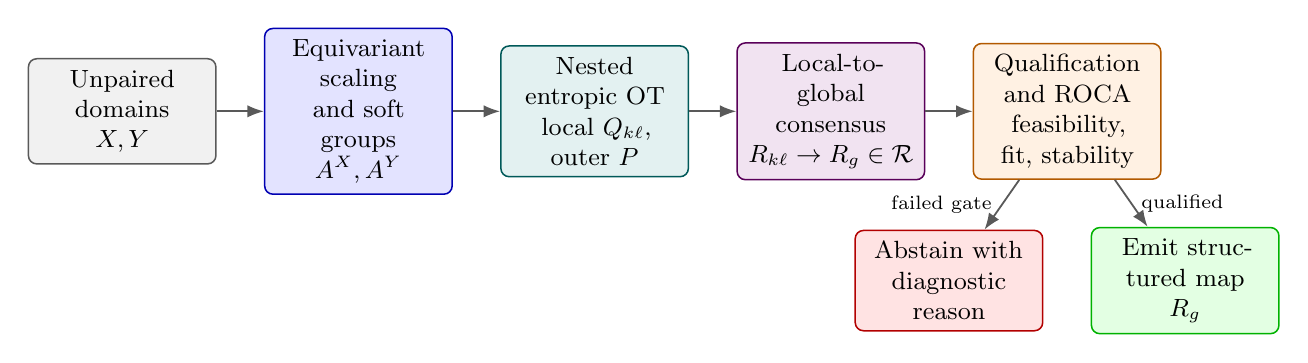
\begin{tikzpicture}[
  font=\small,
  box/.style={draw=#1!70!black, fill=#1!11, rounded corners=3pt, line width=.55pt, align=center, text width=2.1cm, minimum height=1.25cm, inner sep=4pt},
  arrow/.style={-{Latex[length=2.1mm]}, line width=.65pt, draw=black!65}
]
\node[box=gray] (input) at (0,0) {Unpaired domains\\$X, Y$};
\node[box=blue] (groups) at (3.0,0) {Equivariant scaling\\and soft groups\\$A^X, A^Y$};
\node[box=teal] (transport) at (6.0,0) {Nested entropic OT\\local $Q_{k\ell}$, outer $P$};
\node[box=violet] (consensus) at (9.0,0) {Local-to-global consensus\\$R_{k\ell}\rightarrow R_g\in\mathcal R$};
\node[box=orange] (gate) at (12.0,0) {Qualification and ROCA\\feasibility, fit, stability};
\node[box=green] (emit) at (13.5,-2.15) {Emit structured map\\$R_g$};
\node[box=red] (abstain) at (10.5,-2.15) {Abstain with\\diagnostic reason};
\draw[arrow] (input) -- (groups);
\draw[arrow] (groups) -- (transport);
\draw[arrow] (transport) -- (consensus);
\draw[arrow] (consensus) -- (gate);
\draw[arrow] (gate) -- node[right, font=\scriptsize] {qualified} (emit);
\draw[arrow] (gate) -- node[left, font=\scriptsize] {failed gate} (abstain);
\end{tikzpicture}
\caption{GC-HiWA produces a coordinate map only after the structured consensus passes the declared applicability checks. The soft groups and nested transport provide candidate geometric evidence; qualification determines whether that evidence is sufficient to emit $R_g$.}
\label{fig:workflow}
\end{figure}

\subsection{Method lineage and ablation roles}
The final estimator is the endpoint of a method audit, not a relabelling of every exploratory component as a contribution. Table~\ref{tab:en-lineage} records the methods used in this project, the question each was designed to answer, and their evidential status. The MiHiA neural--movement comparison used a fixed, equally sampled $96\times96$ subset and ten independent runs (seeds 80--89). All variants used full-support local transport and the same ADMM convergence requirement; direction labels and movement velocities were opened only after fitting for final scoring. These developmental values illustrate mechanisms and must not be compared directly with the primary synthetic or Panoptic coordinate-recovery results.
\begin{table}[H]\centering\small
\caption{Methods used in the project and their evidential roles. MiHiA values are means over the $96\times96$ neural--movement development subset in ten runs (seeds 80--89); they are not the primary coordinate-recovery validation.}\label{tab:en-lineage}
\begin{tabularx}{\linewidth}{l X X}\toprule
Method & Role and retained mechanism & Audited outcome / interpretation\\\midrule
Hard HiWA & Hard groups, local $Q_{k\ell}$, group $P$, and ADMM consensus \cite{lee2019hierarchical}. & MiHiA development comparison: direction accuracy 0.4188; movement $R^2$ 0.1908.\\
Soft-aggregation HiWA & Prototype-based full-support weighted measures, retaining HiWA transport and consensus \cite{lee2019hierarchical}. & MiHiA development comparison: 0.4271 and 0.1947; retained as a geometric mechanism, not universal transfer.\\
Soft-aggregation HiWA + ROCA & Unlabelled determinant-branch qualification on otherwise comparable candidates. & MiHiA development comparison: 0.4792 and 0.3364; higher-accuracy branch selected in 8/10 runs, so selection is useful but fallible.\\
Component-conditioned local cost & Exploratory $-\beta\log(s_{ij}+10^{-12})$ coupling term. & No stable joint gain; frozen mainline sets $\beta=0$.\\
Unrestricted $O(57)$ & Structural ablation for 19-joint poses. & Did not converge in 100 iterations; rotation error 10.31. It motivates $I_{19}\otimes SO(3)$.\\
GC-HiWA & Soft groups, nested OT, structured consensus and qualification gates. & Primary evidence: 15/15 recoverable acceptances, 25/25 declared-violation abstentions, and controlled Panoptic recovery.\\
\bottomrule\end{tabularx}
\end{table}

\begin{algorithm}[t]\caption{GC-HiWA with qualification}\begin{algorithmic}[1]
\Require Unpaired $X,Y$, declared family $\mathcal R$, group count $K$
\State Normalize each domain; fit soft memberships and build the marginals in Eq.~\ref{eq:en-marginals}
\State Alternate Eq.~\ref{eq:en-inner}, Eq.~\ref{eq:en-outer}, local rotation updates, and Eq.~\ref{eq:en-admm}
\State Check local OT marginals, orthogonality, single-rotation fit, covariance-spectrum necessity, identifiability, and restart stability
\If{any required check fails} \State return \texttt{abstain} with reasons \Else \State qualify determinant candidates with ROCA and return a map only if a healthy candidate exists \EndIf
\end{algorithmic}\end{algorithm}

\Needspace{14\baselineskip}
\begin{samepage}
\subsection{ROCA and the HiWA-based soft-aggregation lineage}
The two connected components of $O(d)$ have determinants $+1$ and $-1$. A low objective can be ambiguous between them. ROCA fits the candidate branches independently. A candidate must converge, pass transport and rotation checks, exhibit a nondegenerate representative-orientation signal, agree with its determinant sign and remain stable across restarts. Only then may ROCA select a branch. Otherwise, it abstains. This is not label-based model selection.

GC-HiWA builds on HiWA's group- and within-group transport, local transformations and global ADMM consensus \cite{lee2019hierarchical}. It introduces prototype-based soft aggregation, full-support weighted measures, the family $I_J\otimes SO(3)$, the transport-weighted structured projection and joint qualification gates for the declared coordinate-recovery task. Earlier exploratory modules are reported only as audited development evidence, not as validated components of the final estimator.
\end{samepage}

\subsection{Four applicability theorems}
The following results place HiWA's correspondence and perturbation conditions together with the structured-map and refusal conditions used here \cite{lee2019hierarchical}. They state when the proposed hierarchy is informative, not that non-convex OT--ADMM always finds a global solution.

\begin{theorem}[Group-correspondence separability]\label{thm:en-correspondence}
Suppose the two domains have $K$ soft-aggregation groups and a true group permutation $\pi$. Let $\widehat C_{k\ell}^{\star}$ be the empirical group-pair cost minimized over the allowed map and local marginals. If, for every $k\ne r$,
\begin{equation}
\widehat C_{k,\pi(r)}^{\star}+\widehat C_{r,\pi(k)}^{\star}-\widehat C_{k,\pi(k)}^{\star}-\widehat C_{r,\pi(r)}^{\star}>E_{k,r}(\delta),
\label{eq:en-exchange-margin}
\end{equation}
where $E_{k,r}(\delta)$ bounds the finite-sample OT error of the four involved soft empirical measures, then the unregularised outer assignment has unique optimum $P_\pi/K$ with probability at least $1-\delta$.
\end{theorem}
For positive outer entropy, this result means that transport mass should concentrate near $P_\pi$, not that the entropic plan is exactly a permutation.

\begin{theorem}[Unique recovery with a correct coupling]\label{thm:en-recovery}
If the declared noiseless model holds, the correct weighted coupling is known, and the weighted source covariance on its support is full rank, the structured Procrustes objective has unique minimiser $R_\star$. For a pose map, it suffices that the joint-aggregated 3-D weighted covariance is full rank.
\end{theorem}

\begin{theorem}[Stability under Gram perturbation]\label{thm:en-stability}
Given the correct group and within-group couplings, form weighted aggregate matrices $X_{\rm agg},Y_{\rm agg}$ and let $\varepsilon^2=\norm{Y_{\rm agg}^\top Y_{\rm agg}-X_{\rm agg}^\top X_{\rm agg}}_F$. If $X_{\rm agg}$ has full row rank, the unconstrained Procrustes minimiser belongs to the declared family $\mathcal R$, and $\varepsilon\norm{X_{\rm agg}^\dagger}\le 2^{-1/2}(\norm{X_{\rm agg}}\norm{X_{\rm agg}^\dagger})^{-1/2}$, then a constant $C_X$ depending only on $X_{\rm agg}$ exists such that
\begin{equation}
\min_{R\in\mathcal R}\norm{Y_{\rm agg}-X_{\rm agg}R^\top}_F^2\le C_X\varepsilon^4.
\label{eq:en-gram-bound}
\end{equation}
\end{theorem}

\begin{theorem}[Refusal boundary from spectral mismatch and symmetry]\label{thm:en-refusal}
An exact orthogonal coordinate map implies equal spectra of the centred, scale-normalised covariances. Hence a nonzero spectral mismatch rules out that exact contract. Conversely, if the covariance is isotropic or has repeated eigenspaces, second-order geometry alone cannot uniquely determine rotations within those eigenspaces.
\end{theorem}
These four conditions motivate the correspondence, full-rank, spectral and identifiability checks used by the qualification gate.

\subsection{Qualification is part of the estimator}
The estimator returns either $(R,\texttt{accepted})$ or $(\varnothing,\texttt{abstain},\texttt{reason})$. Acceptance requires all of the following: local Sinkhorn marginal feasibility, orthogonality of the declared map, a sufficiently small single-rotation residual, compatible covariance-spectrum diagnostics, nondegenerate representative geometry and a stable cluster across independent restarts. A spectrum check is necessary at most; it cannot establish a map by itself. Likewise, a converged OT plan does not establish semantic correspondence.

The one-rotation check compares the cross-domain cost of the final $R_g$ with an internal reference at the same entropy scale. Let $\widehat\pi$ be the Hungarian group matching induced by $P$ and let $\operatorname{OT}_{\varepsilon}$ denote the optimum in Eq.~\ref{eq:en-inner}. We compute
\begin{equation}
\eta=\frac{K_X^{-1}\sum_k\operatorname{OT}_{\varepsilon_{\rm in}}(\alpha^{(k)},\beta^{(\widehat\pi(k))};XR_g^\top,Y)}
{\max\{\tfrac12[L_{X,{\rm self}}+L_{Y,{\rm self}}],10^{-12}\}}.
\label{eq:en-fit-ratio}
\end{equation}
Here $L_{X,{\rm self}}$ and $L_{Y,{\rm self}}$ are the respective averages of same-group, within-domain OT costs. A small $\eta$ indicates that one global rotation is not much worse than within-domain transport. It is a diagnostic, not a semantic-accuracy score or proof of exact recovery.

For the 3-D, four-group ROCA audit, representatives are matched using the candidate group transport and a Hungarian assignment. The sign of the oriented tetrahedral volume
\begin{equation}
V(c_1,c_2,c_3,c_4)=\det[c_2-c_1,\;c_3-c_1,\;c_4-c_1]
\end{equation}
is used only when the simplex is nondegenerate. If two qualified determinant branches disagree and their internal objectives are insufficiently separated, the correct output is abstention rather than a post-hoc accuracy choice.

\section{Evidence protocol}
The primary evidence is frozen and machine-audited. Synthetic generator settings and seeds were fixed before evaluation. Recoverable cases required acceptance and recovery, whereas predeclared mismatch cases required abstention. During Panoptic fitting, extrinsics, synchronized IDs, labels and pairings were masked. They were opened only for post-hoc scoring. The audit script \texttt{experiments/synthetic/verify\_gc\_hiwa\_v2\_evidence.py} checks the cited JSON artefacts.

\begin{table}[t]\centering\small\caption{Primary audited evidence under the stated fitting and evaluation conditions.}\resizebox{\linewidth}{!}{\begin{tabular}{lccc}\toprule
Setting & Runs & Result & Interpretation\\\midrule
Independent recoverable synthetic cases & 15 & 15/15 accepted & Controlled recovery evidence\\
Five declared violation types & 25 & 25/25 abstained & Boundary evidence\\
Isospectral nonorthogonal counterexample & 5 & 5/5 abstained & Spectral equality is insufficient\\
Panoptic qualified recheck & 1 & error 0.00818; R@1=1.0 & Controlled real geometry\\
Panoptic camera configurations & 11 & all converged; max error 0.0308 & Multi-configuration consistency\\
\bottomrule\end{tabular}}\end{table}

\section{Results}
\subsection{Synthetic recovery and rejection}
The independent audit confirmed acceptance in all 15 recoverable cases and abstention in all 25 declared-violation cases, for both core qualification and ROCA. The nonorthogonal isospectral construction had a maximum covariance spectral mismatch of $1.16\times10^{-15}$, yet lacked a single orthogonal ground truth. All five runs abstained because the global single-rotation fit and/or convergence checks failed. Matching covariance spectra are therefore necessary at most, never proof of a common rotation.

Figure~\ref{fig:evidence-summary} visualises the same audited decision outcomes and the controlled Panoptic recheck. The figure separates successful recovery under the declared contract from abstention when the contract is violated. For the Panoptic recheck, post-hoc paired Recall@1 increased from 0.0198 before alignment to 1.0 after applying the qualified map; this quantity is an evaluation-only coordinate-retrieval measure, not a semantic classification score.

\begin{figure}[t]
\centering
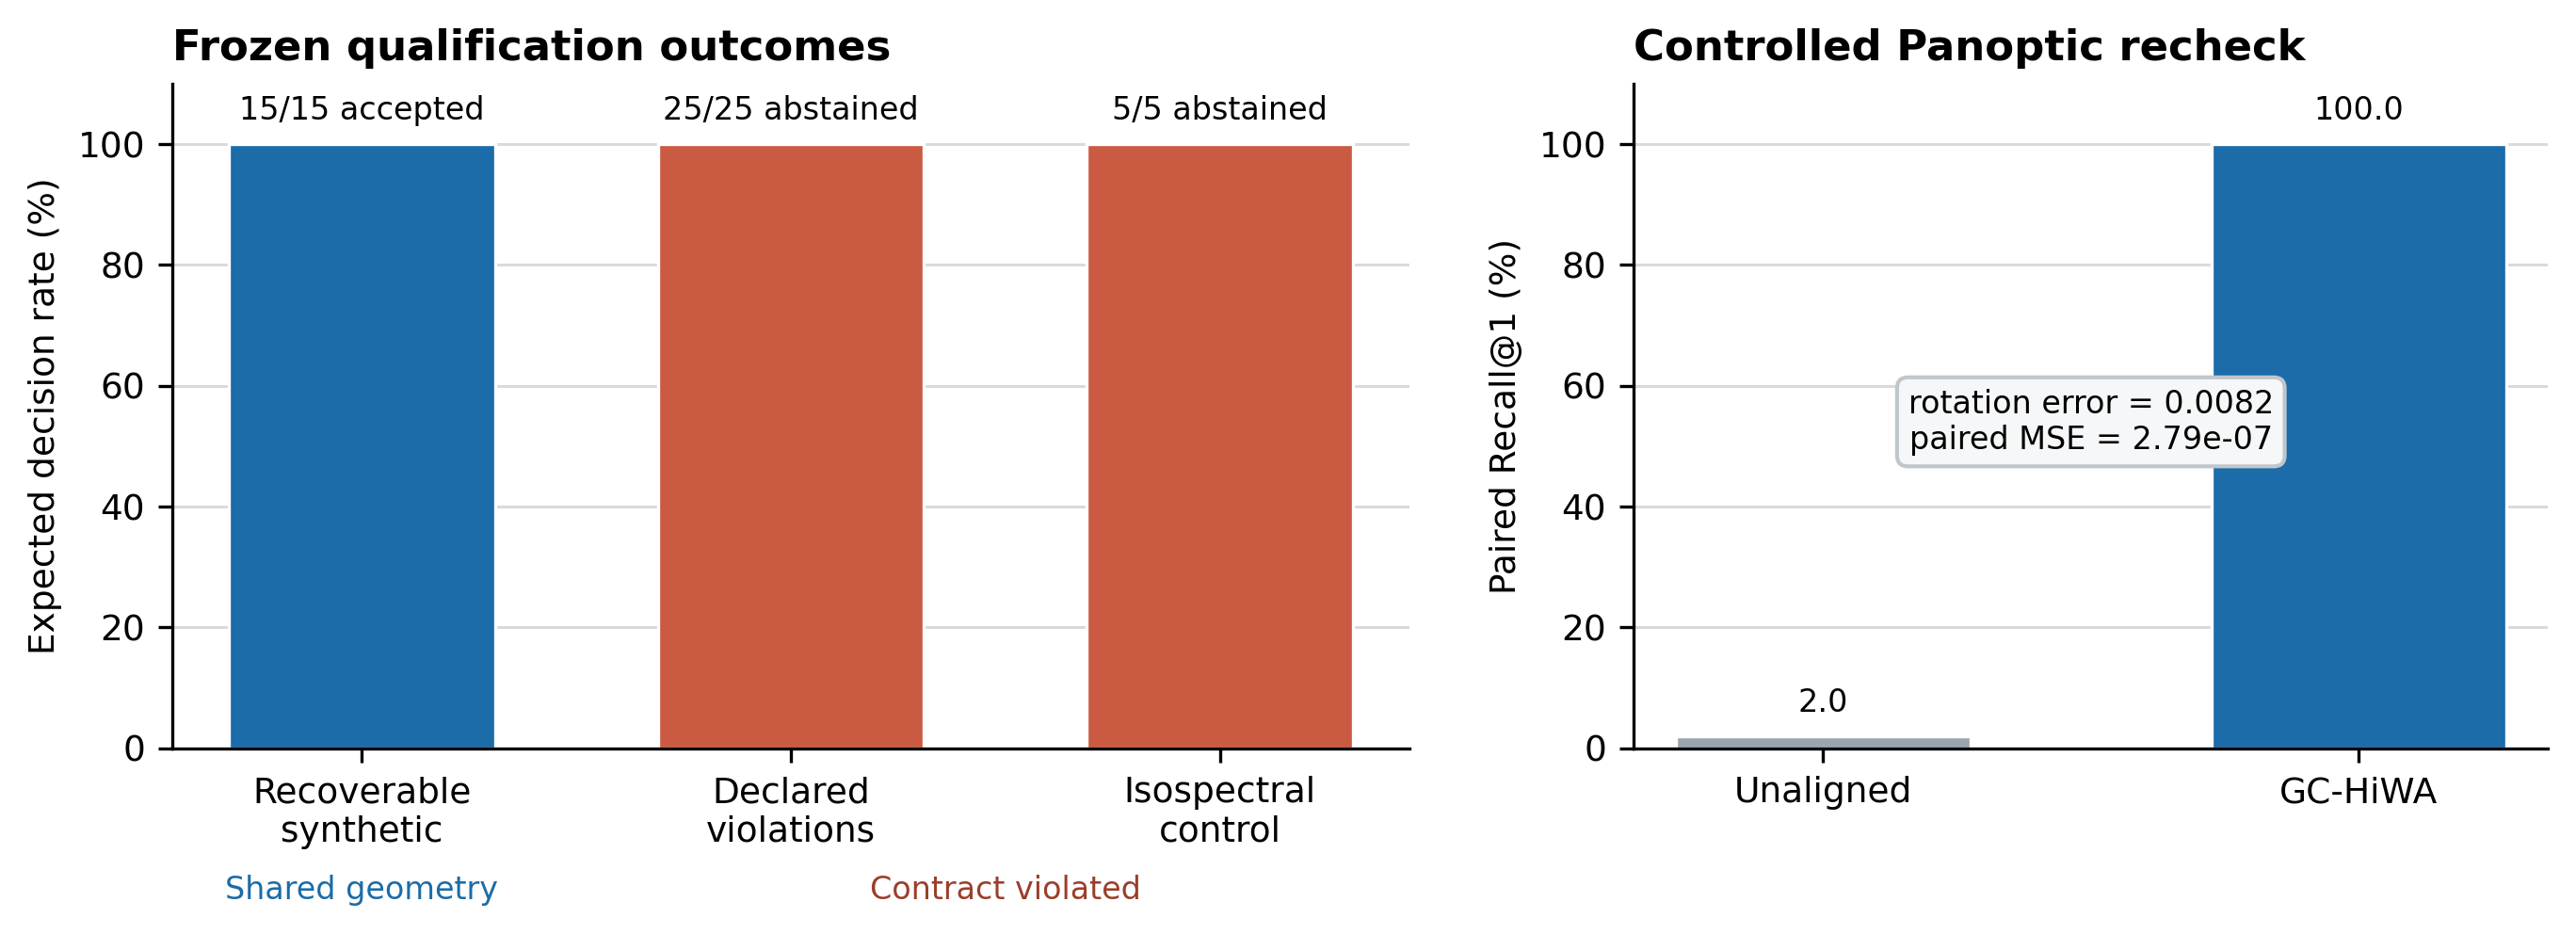
\includegraphics[width=\linewidth]{gc_hiwa_evidence_summary.png}
\caption{Audited evidence summary. \textbf{Left:} expected qualification outcomes on independent synthetic recovery and mismatch cases. \textbf{Right:} post-hoc paired Recall@1 in the controlled Panoptic recheck. The displayed rotation error and paired MSE are evaluation-only quantities.}
\label{fig:evidence-summary}
\end{figure}

\subsection{Controlled Panoptic recovery}
For 19-joint Panoptic skeletons, the structured family has three rotational degrees of freedom, whereas unrestricted $O(57)$ has 1596. The unconstrained model did not converge within the reported 100 iterations and had a rotation error of 10.31. By contrast, the structured camera-pair replicates converged. The primary recheck yielded a Frobenius rotation error of 0.008184, paired alignment MSE of $2.79\times10^{-7}$, an identifiability margin of 0.133 and Recall@1 of 1.0. A frozen, source-defined pose-state proxy also recovered source-model utility on an independent window, from 0.333 before alignment to 0.864 after alignment. This proxy is not an action-recognition result.

\subsection{MiHiA development comparison and external audits}
The MiHiA neural--movement development comparison used an equally sampled $96\times96$ source--target subset. Neural samples supplied the unlabelled alignment inputs; movement-direction labels and continuous movement velocities were not available to prototype fitting, transport, rotation estimation or branch selection. They were opened after these steps to calculate direction accuracy and the coefficient of determination ($R^2$) for velocity prediction. This comparison established a full-support soft-aggregation HiWA baseline and showed why sparse top-membership transport is an approximation, rather than an interchangeable implementation. The baseline uses learned prototypes, row-wise memberships and column-normalized local masses, together with HiWA's uniform-marginal outer coupling $P$, each group-pair coupling $Q_{k\ell}$ and local-to-global rotations. Thus, ``full support'' means that every $Q_{k\ell}$ retains all samples while reweighting their mass. It does not mean that $P$ acquires nonuniform soft-group marginals.

The project also tested a component-conditioned local cost. With group compatibility $s_{ij}=a_i^X P(a_j^Y)^\top$, the exploratory term was $-\beta\log(s_{ij}+10^{-12})$. It allows group compatibility to influence sample transport. It is excluded from the final GC-HiWA backbone because, in neural--movement smoke tests, values that changed continuous $R^2$ reduced direction accuracy, while smaller values yielded no stable joint gain. The final mainline therefore uses $\beta=0$.

Across the ten MiHiA runs (seeds 80--89), Hard HiWA, soft-aggregation HiWA and soft-aggregation HiWA+ROCA achieved mean direction accuracies of 0.4188, 0.4271 and 0.4792. Their movement $R^2$ values were 0.1908, 0.1947 and 0.3364, respectively. ROCA retrospectively selected the higher-accuracy branch in 8 of 10 runs. This is useful, but not error-free, selector evidence. Labels entered stored final metrics only, never memberships, transport or branch selection. These developmental results are distinct from the independent GC-HiWA primary evidence.

\begin{table}[t]\centering\small\caption{MiHiA neural--movement development comparison on the equally sampled $96\times96$ subset, ten runs (seeds 80--89). All methods used full-support transport and the same ADMM convergence requirement; labels were used only for final metrics.}\label{tab:roca}\begin{tabular}{lrr}\toprule
Method & Direction accuracy & Movement $R^2$\\\midrule
Hard HiWA & 0.4188 & 0.1908\\
Soft-aggregation HiWA & 0.4271 & 0.1947\\
Soft-aggregation HiWA + ROCA & \textbf{0.4792} & \textbf{0.3364}\\
\bottomrule\end{tabular}\end{table}

The effect size was heterogeneous. Relative to Hard HiWA, full-support soft aggregation increased mean direction accuracy by 0.0083 and $R^2$ by 0.0039. ROCA increased these quantities by 0.0604 and 0.1456, respectively, but with broad seed variability. Labels appeared only in stored final metrics, never in branch selection. Figure~\ref{fig:roca} shows this distinction.
\begin{figure}[t]\centering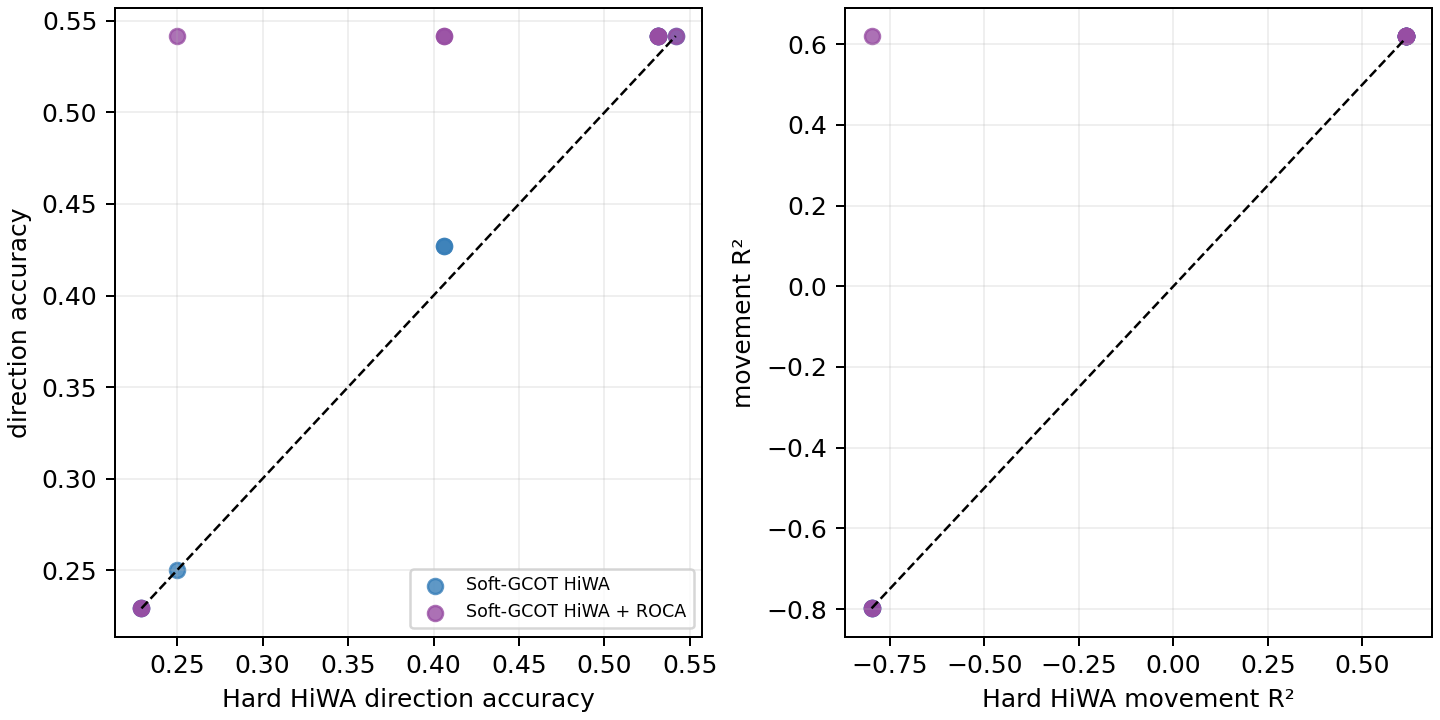
\includegraphics[width=.88\linewidth]{paired_analysis_full_support_roca_seeds_80_89.png}\caption{Paired analysis of the MiHiA $96\times96$ development comparison across ten runs. It is mechanism evidence, not a claim of error-free branch selection.}\label{fig:roca}\end{figure}

Indy-Loco, PBMC RNA--ATAC, PAMAP2 and Paderborn analyses define the limits of the approach. In three Indy-Loco pilots, primal residuals of 4.066, 3.442 and 3.741 exceeded the 0.1 criterion. Paired-oracle checks also did not establish useful transfer. The neural-to-velocity geometry therefore did not satisfy the global-orthogonal contract. PBMC did not yield stable retrieval or cell-type transfer. Paderborn confounded alignment need with entity generalisation, and PAMAP2 showed no stable task-aware OT gain. None of these lines is comparative positive evidence.

\begin{table}[t]\centering\small\caption{Interpretation of all auxiliary data lines.}\begin{tabularx}{\linewidth}{lX}\toprule
Data line & Evidence boundary\\\midrule
Indy-Loco neural-to-velocity & Nonconverged global-rotation OT and weak paired oracle: reject this geometry, do not tune OT parameters further.\\
PBMC RNA--ATAC & Shared features did not yield stable retrieval or label transfer; not a positive alignment result.\\
Paderborn bearing & The available splits either remove the alignment need or confound entity generalization.\\
PAMAP2 sensors & Task-aware OT did not give a stable, multi-subject gain.\\
\bottomrule\end{tabularx}\end{table}

\section{Discussion and limitations}
GC-HiWA does not claim universal improvement. Its contribution is to formalise when an unsupervised alignment has sufficient numerical and geometric support to be emitted. The recovery theorem assumes a correct coupling and full-rank geometry; it is not a global convergence proof for the complete OT--ADMM problem. The thresholds are fixed engineering diagnostics, not distribution-wide error guarantees. Panoptic provides controlled, same-system geometry, and the source-defined pose-state proxy is not independently labelled semantic-action transfer. The appropriate next test is a preregistered, subject-disjoint semantic-action protocol. Until then, no cross-device semantic-generalisation claim is warranted.

\section{Data sources, use, and evidence boundary}
\textbf{Synthetic data} were generated as 3-D grouped point sets under either the declared single-rotation contract or a predeclared violation; they test recovery and abstention only. \textbf{Panoptic Studio data} were 19-joint 3-D skeletons from camera pairs in one capture system; extrinsics, synchronized-frame identities and labels were hidden during fitting and opened only for post-hoc coordinate scoring. \textbf{MiHiA neural--movement data} supplied the $96\times96$ development comparison described above; its direction and velocity outcomes were evaluation-only. \textbf{Indy-Loco, PBMC RNA--ATAC, PAMAP2 and Paderborn} were examined exclusively as applicability-boundary data lines: their results are reported to explain why they do not support a positive transfer claim. No result in this paper establishes semantic action recognition or universal cross-device generalisation.

\section{Reproducibility}
The core implementation is in \url{src/cc_hiwa/}. The synthetic runner is \url{experiments/synthetic/run_gc_hiwa_boundary_benchmark.py}, Panoptic runners are in \url{experiments/panoptic/}, and frozen artefacts are in \url{experiments/results/}.\\
The evidence audit passed against the current artefact set. The documented Windows test configuration sets \texttt{OMP\_NUM\_THREADS=1} and \texttt{MKL\_NUM\_THREADS=1} only to avoid an intermittent runtime abort. It does not change algorithmic parameters.

\section{Conclusion}
GC-HiWA casts unpaired coordinate alignment as conditional recovery. Its soft aggregation and HiWA-style hierarchical transport provide the alignment structure. ROCA and the applicability gates prevent ambiguous or mismatched inputs from being reported as successful mappings. Synthetic boundary tests and controlled multi-camera pose recovery support this narrow claim, while the MiHiA development comparison and external negative results define its limits.
\appendix
\section{Notation}
\begin{longtable}{p{0.35\linewidth}p{0.57\linewidth}}
\toprule Symbol & Meaning\\\midrule
\endfirsthead\toprule Symbol & Meaning\\\midrule\endhead
$X,Y;\ n,m,d$ & Unpaired source and target sample matrices; their sample counts and common feature dimension.\\
$Z_X,Z_Y;\ C^X,C^Y;\ c_k^X,c_\ell^Y$ & Globally centred and scaled samples; prototype matrices; and their prototype rows.\\
$A^X,A^Y;\ a_{ik}^X,a_{j\ell}^Y;\ K_X,K_Y;\tau_X,\tau_Y$ & Soft-membership matrices and entries; group counts; and membership temperatures.\\
$\alpha^{(k)},\beta^{(\ell)};\ Q_{k\ell};\ P;\mathcal V$ & Normalised local marginals; local sample transport; outer group transport; and its uniform-marginal feasible set.\\
$R_\star,R_{k\ell},R_g;\mathcal R;\Pi_{\mathcal R};\Lambda_{k\ell}$ & True map for evaluation, local rotations, emitted rotation, allowed family, projection, and scaled ADMM multiplier.\\
$I_J;\SO(3);O(d)$ & Identity of joint-block size $J$, proper 3-D rotations, and the full orthogonal group in dimension $d$.\\
$D^{(k\ell)},C_{k\ell};\varepsilon_{\rm in},\varepsilon_{\rm out};\rho;w_{k\ell}$ & Local squared-distance cost, group-pair cost, entropy strengths, ADMM penalty, and transport weight.\\
$s_{ij};\beta;\lambda_H,\lambda_2$ & Component compatibility, its exploratory weight, and prototype entropy/scale weights.\\
$\pi,\widehat\pi;\eta;\delta_{\rm spec};\kappa_{\rm id}$ & Latent and estimated group permutations; single-rotation fit ratio; spectral diagnostic; and identifiability margin.\\
$P_\pi;E_{k,r}(\delta);\delta$ & Permutation plan, finite-sample group-cost error bound, and its probability level.\\
$\varepsilon;X_{\rm agg},Y_{\rm agg};X_{\rm agg}^{\dagger};C_X$ & Gram-perturbation magnitude, weighted aggregates, Moore--Penrose pseudoinverse, and the stability-bound constant.\\
\bottomrule
\end{longtable}
\bibliographystyle{plain}\bibliography{references}
\end{document}
